\documentclass[10pt,landscape,a4paper]{article}
\usepackage[utf8]{inputenc}
\usepackage[english]{babel}
\usepackage[utopia,sfscaled]{mathdesign}
\usepackage{multicol}
\usepackage[top=2mm,bottom=2mm,left=2mm,right=2mm]{geometry}
\usepackage{lipsum}
\usepackage[framemethod=tikz]{mdframed}
\usepackage{microtype}
\usepackage{graphicx}
\usepackage{amsmath}
\usepackage{breqn}
\usepackage{enumitem}
\usepackage{titlesec}

\setitemize{noitemsep,topsep=0pt,parsep=0pt,partopsep=0pt}
\setenumerate{noitemsep,topsep=0pt,parsep=0pt,partopsep=0pt}
\setlength{\parindent}{0pt}
\setlength{\parskip}{0.2\baselineskip}
\titleformat*{\section}{\footnotesize\bfseries}
\titleformat*{\subsection}{\scriptsize\bfseries}
\titlespacing{\section}{0pt}{\parskip}{-\parskip}
\titlespacing{\subsection}{0pt}{\parskip}{-\parskip}

\graphicspath{{images/}}

\newcommand*{\vertbar}{\rule[-1ex]{0.5pt}{2.5ex}}
\newcommand*{\horzbar}{\rule[.5ex]{2.5ex}{0.5pt}}

\DeclareMathOperator*{\argmin}{argmin}
\DeclareMathOperator*{\argmax}{argmax}
\DeclareMathOperator*{\composition}{I}

%%%%%%%%%%%%%%%%%%%%%%%%%%%%%%%%%%%%%%%%%%%%%
%%%%%%%%%%%%%%%%%%%%%%%%%%%%%%%%%%%%%%%%%%%%%
%%%%%%%%%%%%%%%%%%%%%%%%%%%%%%%%%%%%%%%%%%%%%
%%%%%%%%%%%%%%%%%%%%%%%%%%%%%%%%%%%%%%%%%%%%%
%%%%%%%%%%%%%%%%%%%%%%%%%%%%%%%%%%%%%%%%%%%%%
%%%%%%%%%%%%%%%%%%%%%%%%%%%%%%%%%%%%%%%%%%%%%
%%%%%%%%%%%%%%%%%%%%%%%%%%%%%%%%%%%%%%%%%%%%%
%%%%%%%%%%%%%%%%%%%%%%%%%%%%%%%%%%%%%%%%%%%%%
%%%%%%%%% CODE APPEARANCE CONFIG %%%%%%%%%%%%
%%%%%%%%%%%%%%%%%%%%%%%%%%%%%%%%%%%%%%%%%%%%%
%%%%%%%%%%%%%%%%%%%%%%%%%%nicolas igor %%%%%%

%%%%%%%%%%%%%%%%% README %%%%%%%%%%%%%%%%%%%%
% This is a config file to set:
%   1. Style for listing package (could be use on any language)
%   2. Julia syntax highlighting definition
%   3. Command and environment to insert julia, python, and matlab code in your document easily.
%
%       a. new commands: \juliaFile, \pythonFile, and \matlabFile
%           All three are used like \juliaFile[folder_name]{file_name}
%           folder_name is optional, and do it with the slash, e.g. "myFolder/". When no folder is provided, it is assumed that the code is in the same directory as your document.
%           For file_name, do it without extension (it is assumed).
%       Example:
%           \juliaFile[codes/]{kMeans}
%           \juliaFile{randomForest}
%
%       b. new environments: if you want to write your code directly in your document. juliaText, pythonText, and matlabText are provided. Example:
%           \begin{juliaText}{Write your caption here.}
%           Write your code here
%           \end{juliaText}
%%%%%%%%%%%%%%%%%%%%%%%%%%%%%%%%%%%%%%%%%%%%



% Better font encoding, and customized fixed-width font
\usepackage[T1]{fontenc}
\usepackage{inconsolata}

% Colors Definition for Listing Highlighting
\usepackage{color}
\definecolor{codeRed}{rgb}{0.5,0,0}
\definecolor{codeGreen}{rgb}{0,0.6,0}
\definecolor{codeBlue}{rgb}{0,0,0.5}
\definecolor{codeGray}{rgb}{0.5,0.5,0.5}
\definecolor{codeMauve}{rgb}{0.58,0,0.82}

%%%%%%%%%%%%%%%%%%%%%%%%%%%%%%%%%%%%%%%%%%%%%
%%%%%%%%% LISTING FUN STARTS HERE!!! %%%%%%%%
%%%%%%%%%%%%%%%%%%%%%%%%%%%%%%%%%%%%%%%%%%%%%
\usepackage{listings} % For displaying code

% General Appearance Settings in an Isolated Style
\lstdefinestyle{myStyle}{ %
  basicstyle=\tiny\ttfamily,      % the size of the fonts that are used for the code
  basewidth=0.5em,                 % sets size of reserved space on each column
  breakatwhitespace=true,          % sets if automatic breaks should only happen at whitespace
  breaklines=true,                 % sets automatic line breaking
  commentstyle=\color{codeGreen},  % comment style
  extendedchars=true,              % lets you use non-ASCII characters; for 8-bits encodings only, does not work with UTF-8
  frame=tb,	                       % adds a frame around the code
  keywordstyle=\color{codeBlue},       % keyword style
  numbers=none,                    % where to put the line-numbers; possible values are (none, left, right)
  numbersep=5pt,                   % how far the line-numbers are from the code
  numberstyle=\scriptsize\color{codeGray}, % the style that is used for the line-numbers
  rulecolor=\color{black},         % if not set, the frame-color may be changed on line-breaks within not-black text (e.g. comments (green here))
  showspaces=false,                % show spaces everywhere adding particular underscores; it overrides 'showstringspaces'
  showstringspaces=false,          % underline spaces within strings only
  showtabs=false,                  % show tabs within strings adding particular underscores
  stepnumber=1,                    % the step between two line-numbers. If it's 1, each line will be numbered
  numberfirstline=true,
  numberblanklines=true,
  stringstyle=\color{codeMauve},     % string literal style
  tabsize=4,	                   % sets default tabsize to 4 spaces
}

% Definition of Julia Highlighting
\lstdefinelanguage{Julia}%
{ language = Matlab,%
    keywordsprefix=\@,%
    morekeywords={
    exit,whos,edit,load,is,isa,isequal,typeof,tuple,ntuple,uid,hash,finalizer,convert,promote,
    subtype,typemin,typemax,realmin,realmax,sizeof,eps,promote_type,method_exists,applicable,
    invoke,dlopen,dlsym,system,error,throw,assert,new,Inf,Nan,pi,im,begin,while,for,in,return,
    break,continue,macro,quote,let,if,elseif,else,try,catch,end,bitstype,call,do,using,module,
    import,export,importall,baremodule,immutable,local,global,const,Bool,Int,Int8,Int16,Int32,
    Int64,Uint,Uint8,Uint16,Uint32,Uint64,Float32,Float64,Complex64,Complex128,Any,Nothing,nothing,
    function,type,typealias,abstract,case,false,otherwise,switch,true,include
  },%
  sensitive=true, %
  comment=[l]{\#}, % l is for line comment
  morecomment=[s]{\#=}{=\#}, % s is for start and end delimiter
  string=[b]" % defines that strings are enclosed in double quotes
}

% Command to include files of code easier, Julia
\newcommand{\juliaFile}[2][]{\lstinputlisting[caption=Script \emph{#2}., label=code:#2, style=myStyle, language=Julia]{#1#2.jl}}
% Command to include files of code easier, Python
\newcommand{\pythonFile}[2][]{\lstinputlisting[caption=Script \emph{#2}., label=code:#2, style=myStyle, language=Python]{#1#2.py}}
% Command to include files of code easier, Matlab
\newcommand{\matlabFile}[2][]{\lstinputlisting[caption=Script \emph{#2}., label=code:#2, style=myStyle, language=Matlab]{#1#2.m}}

% Environment to write by hand code easier, Julia
\lstnewenvironment{juliaText}[1]{\lstset{caption=#1, style=myStyle, language=Julia, firstnumber=1}}{}
% Environment to write by hand code easier, Python
\lstnewenvironment{pythonText}[1]{\lstset{caption=#1, style=myStyle, language=Python, firstnumber=1}}{}
% Environment to write by hand code easier, Matlab
\lstnewenvironment{matlabText}[1]{\lstset{caption=#1, style=myStyle, language=Matlab, firstnumber=1}}{}

%%%%%%%%%%%%%%%%%%%%%%%%%%%%%%%%%%%%%%%%%%%%%
%%%%%%%%%%% LISTING FUN ENDED  %%%%%%%%%%%%%%
%%%%%%%%%%%%%%%%%%%%%%%%%%%%%%%%%%%%%%%%%%%%%


\begin{document}
\tiny
\begin{multicols*}{5}
\section{Validation}
% TODO: 2016_valid Q1 pseudocode

Validation Techniques:
\begin{itemize}
    \item fixed-validation:
    \begin{itemize}
        \item fixed sizes of train dataset and validation dataset
    \end{itemize}
    \item k-fold validation:
    \begin{itemize}
        \item divide dataset into \(k\) parts
        \item use \(k-1\) parts for training and the other part for validation
        \item repeat \(k\) times then average
    \end{itemize}
    \item loop validation (leave-one-out validation):
    \begin{itemize}
        \item use all dataset for training but leave one object for validation
        \item repeat \(n\) times then average
    \end{itemize}
\end{itemize}
Model Selection:
\begin{itemize}
    \item optimization bias is small when a few models are compared
    \item optimization bias is large when a lot of models are compared
\end{itemize}


\section{Parametric \& Non-Parametric}
\begin{itemize}
    \item parametric
    \begin{itemize}
        \item fixed \# parameters
        \item more data doesn't help
    \end{itemize}
    \item non-parametric
    \begin{itemize}
        \item \# parameters grows with \(n\)
        \item more data \(\rightarrow \)  more complicated
    \end{itemize}
    \item examples:
    \begin{itemize}
        \item k-means (non-parameters)
        \item softmax multi-class classification (parametric)
        \item PCA (parametric)
        \item neural networks (parametric)
    \end{itemize}
\end{itemize}

\section{Data Standardization}
\begin{itemize}
    \item \(\mu \) = mean of \(X_j\) and \(y\), \(\sigma \) = std of \(X_j\) and \(y\)
    \item \(x_i = x_i - \frac{\mu}{\sigma}\)
    \item use the \(\mu \) and \(\sigma \) from training data on test data
\end{itemize}

\section{Feature Selection}

Note:
Regression Weights vs. Search and score
\begin{itemize}
    \item pro: fast
    \item con: may drop import features if collinear
\end{itemize}

\section{Decision Tree}
Decision Stump: (\(n\) objects, \(d\) features, \(t\) thresholds)
\begin{itemize}
    \item cost:
    \begin{itemize}
        \item cost: \(O(ndt)\) (without sorting, computing score for \(dt\) rules)
        \item cost: \(O(n^2d)\) (consider only features)
        \item cost: \(O(nd \log(n))\) (with sorting, sorting costs \(O(n \log(n))\) per feature)
    \end{itemize}
\end{itemize}

\section{Naïve Bayes}
\begin{align*}
    p(y_i|x_i) &= \frac{p(x_i|y_i) p(y_i)}{p(x_i)} \\
    &\propto p(x_i|y_i) p(y_i) \\
    &\approx \prod_{j=1}^{d} (p(x_{ij}|y_i)) p(y_i)
\end{align*}
\begin{equation*}
    p(\hat{y} = 1|\hat{x}) > p(\hat{y}=0|\hat{x}) \Rightarrow \hat{y} = 1
\end{equation*}

\subsection{Note}
Laplace Smoothing:\(\frac{(\text{\# spam messages with } x_i)+1}{(\text{\# spam messages})+2}\) \\
Decision Theory: assign a cost to each scenario

\section{K-Nearest Neighbours (KNN)}
KNN
\begin{itemize}
    \item non-parametric (size of model = \(O(nd)\))
    \item no training phase
    \item expansive prediction (\(O(nd)\) for 1 test object)
\end{itemize}
KNN Procedure:
\begin{enumerate}
    \item find \(k\) training examples \(x_i\) that are most similar to \(\hat{x}\) in terms of Euclidean distance
    \item classify using the most common label of similar examples
\end{enumerate}

\subsection{Note}
Problems:
\begin{itemize}
    \item exponentially more points needed when dimensions grows
    \item can be problematic when features have different scales
\end{itemize}

\section{Ensemble Methods}
Ensemble Methods
\begin{itemize}
    \item classifiers that take other classifiers as input.
    \item do much better than a single classifier
\end{itemize}
Two Types of Ensemble Methods:
\begin{itemize}
    \item Boosting --- improves \(E_{train}\) of classifiers with high \(E_{train}\)
    \item Averaging --- improves \(E_{approx}\) of classifiers with high \(E_{approx}\)
    \begin{enumerate}
        \item take predictions from a set of models as input
        \item take mode of predictions as output
    \end{enumerate}
\end{itemize}

\subsection{Random Forests}
Bootstrapping
\begin{juliaText}{}
for i in 1:n
    j = rand(1:n)
    X_bootstrap[1,:] = X[j,:]
\end{juliaText}
\begin{enumerate}
    \item generate several bootstrap examples
    \item fit a classifier to each bootstrap sample
    \item average predictions at test time
\end{enumerate}
Random Trees
\begin{itemize}
    \item use a subset of features for each random tree
    \item each decision stump considers a randomly-chosen feature
\end{itemize}

\section{Clustering}

\subsection{K-Means}
K-Means Input
\begin{itemize}
    \item \# clusters \(k\)
    \item initial guess of the mean of each cluster
\end{itemize}
Procedure
\begin{enumerate}
    \item assign each \(x_i\) to its closest mean
    \item update means
    \item repeat until convergence
\end{enumerate}
Cost
\begin{itemize}
    \item \(O(d)\) --- compute the Euclidean distance between \(x_i\) and each mean \(w_c\)
    \item \(O(ndk)\) --- assign objects to different clusters
    \item \(O(nd)\) --- update a mean
\end{itemize}
Vector Quantization \\
Replace objects with its cluster mean \\
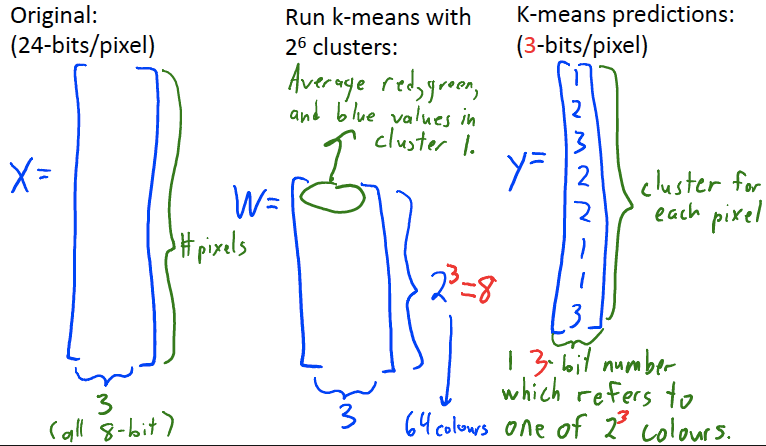
\includegraphics[scale=0.2]{vector_quantization}
Problems
\begin{itemize}
    \item assume \(k\) is known
    \item no overlapping or unassigned objects
    \item may converge to sub-optimal solution
    \item can't deal with non-convex data properly
\end{itemize}

\subsection{Density-Based Clustering}
Two Hyperparameters
\begin{itemize}
    \item radius --- min distance between closed points
    \item minPoints --- \# reachable points (core)
\end{itemize}
Procedure
\begin{enumerate}
    \item if \(x_i\) already assigned to a cluster, do nothing
    \item check if \(x_i\) is a core point
    \begin{itemize}
        \item yes \(\rightarrow \) expand cluster
        \begin{enumerate}[label=\arabic*]
            \item assign all \(x_j\) with distance \(r\) of core point \(x_i\) to cluster
            \item for each newly-assigned \(x_j\) that is core point, expand cluster
        \end{enumerate}
        \item no  \(\rightarrow \) do nothing
    \end{itemize}
\end{enumerate}
Problems
\begin{itemize}
    \item some points not assigned
    \item ambiguity of non-core (boundary) points
    \item sensitive to choice of radius and minPoints
    \begin{itemize}
        \item not sensitive to initialization (expect for boundary points)
    \end{itemize}
    \item finding cluster is expansive when a new example added
    \begin{itemize}
        \item need to compute distances to training points
    \end{itemize}
    \item need a lot of points to fill the space in high dimensions
\end{itemize}
Label Switching Problem \\
\begin{itemize}
    \item cluster labels \(y_i\) are meaningless
    \item same clustering with permuted labels
    \item all \(y_i\) become equally likely as \# initializations inceases
\end{itemize}

\subsection{Hierarchical Clustering}
Density-Based Hierarchical Clustering
\begin{itemize}
    \item fixed radius
    \item vary minPoints
\end{itemize}
Agglomerative (Bottom-Up) Clustering \\
\underline{Procedure}
\begin{enumerate}
    \item start with each point in its own cluster
    \item each step merges the two closest clusters
    \item stop when when every thing in one big cluster
\end{enumerate}
\underline{Cost} \(O(n^3d)\)

\subsection{Outliler Detection}
Model-Based \\
\underline{Procedure}
\begin{itemize}
    \item fit a probabilistic model
    \item outliers have low probability
\end{itemize}
\underline{Problems}
\begin{itemize}
    \item mean and var sensitive to outliers
    \item alternative: quantiles/sequentially remove worse outlier
    \item hard to define outliers (global vs. local outliers)
\end{itemize}
Graphical \\
\underline{Procedure}
\begin{itemize}
    \item look at a plot of the data
    \item outliers decided by humans
\end{itemize}
% TODO: Add graphical outlier detection examples
Cluster-Based \\
\underline{Procedure}
\begin{enumerate}
    \item cluster the data
    \item find the points that don't belong to a cluster
\end{enumerate}
% TODO: Add cluster-based outlier detection examples
Supervised Outlier Detection \\
\underline{Problems}
\begin{itemize}
    \item need to know what outliers look like
    \item may not detect new types of outliers
\end{itemize}

\subsection{\emph{Note}}
Density-Based vs. K-Means:
\begin{itemize}
    \item pros:
    \begin{itemize}
        \item don't need to pre-specify \# clusters
    \end{itemize}
    \item cons:
    \begin{itemize}
        \item no loss function interpretation
        \item two hyper parameters to set
        \item slower \& more complicated
    \end{itemize}
\end{itemize}

\section{Regression}

\subsection{Linear Regression}
Change of Basis
\begin{dmath*}
    Z =
    \begin{bmatrix}
        1 & x_{11} & \cdots & x_{1n} \\
        1 & x_{21} & \cdots & x_{2n} \\
        \vdots & \vdots & \vdots & \vdots \\
        1 & x_{n1} & \cdots & x_{nn} \\
    \end{bmatrix}
\end{dmath*}

\subsection{Polynomial Regression}
Change of Basis
\begin{dmath*}
    Z =
    \begin{bmatrix}
        1 & x_1 & x_1^2 & x_1^p \\
        1 & x_2 & x_2^2 & x_2^p \\
        \vdots & \vdots & \vdots & \vdots \\
        1 & x_n & x_n^2 & x_n^p \\
    \end{bmatrix}
\end{dmath*}

\subsection{Robust Regression}
\begin{dmath*}
    f(w) = \sum_{i=1}^{n} |w^\intercal x_i - y_i| = ||Xw - y||_1
\end{dmath*}
\begin{itemize}
    \item less sensitive to outliers
\end{itemize}
Smooth Approximation \\
\underline{Huber Loss} \\
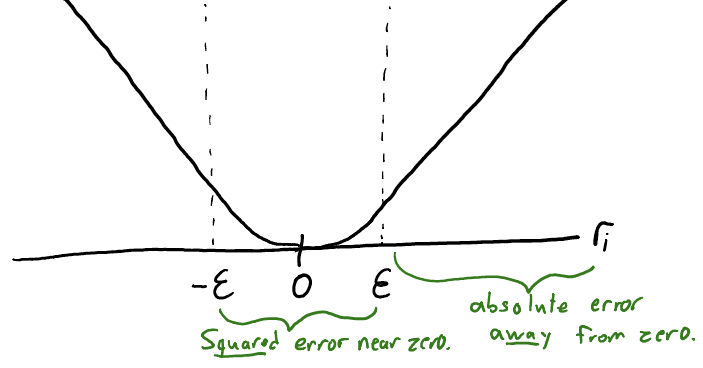
\includegraphics[scale=0.2]{huber_loss}
\begin{align*}
    f(w) &= \sum_{i=1}^{n} h(x^\intercal x_i - y_i) \\
    h(r_i) &=
    \begin{cases}
        \frac{1}{2}r_i^2 \text{ for \(|r_i| \leq \epsilon \)}\\
        \epsilon (|r_i|-\frac{1}{2} \epsilon) \text{ otherwise}
    \end{cases}
\end{align*}

\subsection{Brittle Regression}
\begin{dmath*}
    f(w) = ||Xw - y||_{\infty}
\end{dmath*}
Smooth Approximation \\
\underline{Log-Sum_Exp}
\begin{dmath*}
    \max_i \{z_i\} \approx \log(\sum_i \exp(z_i))
\end{dmath*}

\subsection{Finding \(w\)}
\begin{dmath*}
    (X^\intercal X) w = X^\intercal y
\end{dmath*}
Cost
\begin{itemize}
    \item \(O(nd^2)\) --- \(X^\intercal X\)
    \item \(O(nd)\) --- \(X^\intercal y\)
    \item \(O(d^3)\) --- solve \(d \times d\) system
    \item \(O(nd^2 + d^3)\) --- total
\end{itemize}
Alternative: gradient descent

% TODO: L16 Complexity Pentalties

\section{Gaussian RBFs}
Radial Basis Functions (RBFs)
\begin{dmath*}
    Z =
    \begin{bmatrix}
        g(||x_1-x_1||) & g(||x_1-x_2||) & \cdots & g(||x_1-x_n||) \\
        g(||x_2-x_1||) & g(||x_1-x_2||) & \cdots & g(||x_2-x_n||) \\
        \vdots & \vdots & \ddots & \vdots \\
        g(||x_n-x_1||) & g(||x_n-x_2||) & \cdots & g(||x_n-x_n||)
    \end{bmatrix}_{n \times n}
\end{dmath*}
Gaussian RBF: \(g(\delta) = \exp(-\frac{\delta^2}{2\sigma^2})\)
\begin{itemize}
    \item \(\sigma^2\) = hyperparameter controlling the width, which affect the fundamental trade-off
\end{itemize}
Predictions
\begin{dmath*}
    \hat{Z} =
    \begin{bmatrix}
        &  &  & \\
    & g(||\hat{x_i}-x_j||) &  &  \\
        &  &  &  \\
    &  &  &
\end{bmatrix}_{n \times t}
\end{dmath*}
Regularization: L2 regularization
Choosing \(\sigma \) \& \(\lambda \): cross-validation

\section{Gradient Descent}
Procedure
\begin{enumerate}
    \item start with initial guess \(w^0\)
    \item \(w^1 = w^0 - \alpha^0 \nabla f(w^0)\)
    \item \(w^{t+1} = w^t - \alpha^t \nabla f(w^t)\)
\end{enumerate}
Cost (compute \(\nabla f(w) = X^\intercal Xw - X^\intercal y\))
\begin{itemize}
    \item \(O(nd)\) --- \(Xw\)
    \item \(O(nd)\) --- \(X^\intercal Xw\)
    \item \(O(nd)\) --- \(X^\intercal y\)
    \item \(O(ndt)\) --- total
\end{itemize}

\section{Stochastic Gradient Descent}
Procedure
\begin{enumerate}
    \item start with initial guess \(w^0\)
    \item \(w^1  = w^0 - \alpha^0 \nabla f_i(w^0)\)
    \item \(w^{t+1} = w^t - \alpha^t \nabla f_i(w^t)\)
\end{enumerate}
\begin{itemize}
    \item random example \(i\)
    \item \(\nabla f(w^t) = \frac{1}{n} \sum_{i=1}^{n} \nabla f_i(w^t)\)
\end{itemize}

\subsection{Variance of Random Gradients}
\begin{dmath*}
    \frac{1}{n} \sum_{i=1}^{n} ||\nabla f_i(w^t) - \nabla f(w^t)||^2
\end{dmath*}
\begin{itemize}
    \item variance = 0 \(\rightarrow \) every step goes in the right direction \(\Rightarrow \)  outside of region of confusion
    \item variance is small \(\rightarrow \) most steps go in the right direction \(\Rightarrow \)  just inside region of confusion
    \item variance is large \(\rightarrow \) many steps go in the wrong direction \(\Rightarrow \) middle of region of confusion, where \(w^*\) lives
\end{itemize}

\subsection{Effect of Step-Size}
Step-size \(\downarrow \rightarrow \) effect of variance \(\downarrow \) \\
For a fixed step-size, SG makes progress until variance is too big
\begin{itemize}
    \item rapid progress --- when far from solution
    \item erratic hehaviour --- confined to a ``ball'' around solution
    \begin{itemize}
        \item radius of ball \(\propto \) step-size
    \end{itemize}
\end{itemize}
Choosing step-size
\begin{itemize}
    \item must satisfy \(\sum_{t=1}^{\infty} \alpha^t = \infty\) \& \(\sum_{t=1}^{\infty} (\alpha^t)^2 < \infty\)
    \item can achieve by using a step-size sequence like \(\alpha^t = O(\frac{1}{t})\)
    \item in practice: add extra parameters \(\alpha^t = \frac{\beta}{(t+\gamma)}\)
\end{itemize}

\subsection{\emph{Note}}
\begin{itemize}
    \item minibatch size \(\downarrow \) \(\rightarrow \) each iteration is faster, but more iterations needed
\end{itemize}

\section{Feature Selection}

\subsection{Regression Weight}
Procedure
\begin{enumerate}
    \item fit regression weights \(w\)
    \item takes features \(j\), where \(|w_j| > \text{a threshold }\)
\end{enumerate}
Problems
\begin{itemize}
    \item collinearity --- one/both/none will be taken
\end{itemize}

\subsection{Search and Score}
Procedure
\begin{enumerate}
    \item define score function \(f(s)\) that measures quality of set of features \(S\)
    \item search for \(S\) with best score
\end{enumerate}
Score Function
\begin{itemize}
    \item can't be \(E_{train}\) since it goes down as more features added
    \item \(E_{valid}\) is a good choice
\end{itemize}
Problems
\begin{itemize}
    \item large \# sets (\(2^d\) sets)
    \item high optimization bias
    \item prone to false positives
\end{itemize}
Non-Zero Penalties
\begin{dmath*}
    score(S) = \frac{1}{2} \sum_{i=1}^{n} (w_s^\intercal x_{is} - y_i)^2 + size(S)
\end{dmath*}
\begin{itemize}
    \item L0-norm can be used for \(size(S)\)
\end{itemize}

\subsection{Feature Selection Guide}
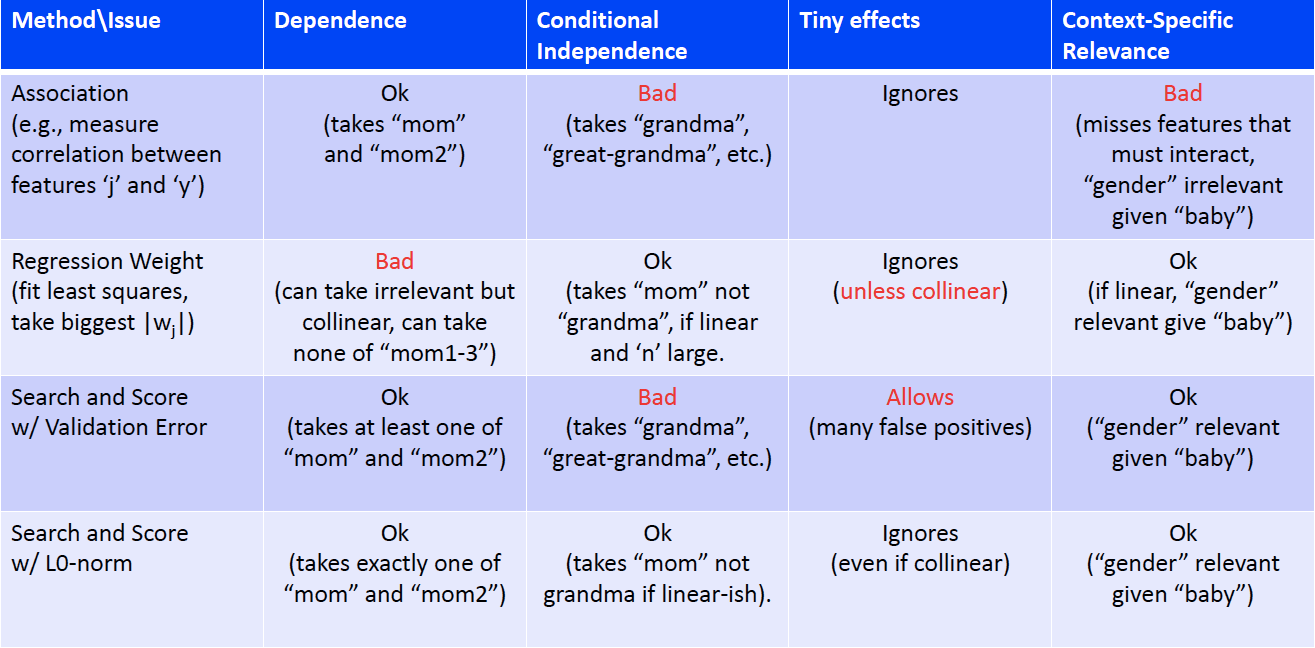
\includegraphics[scale=0.12]{feature_selection_guide}

\subsection{Ensemble Feature Selection}
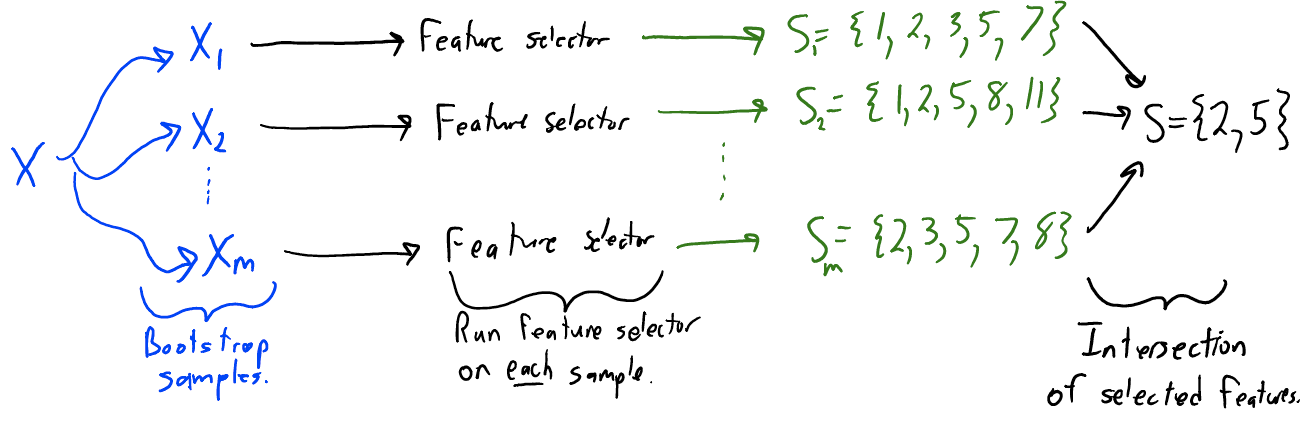
\includegraphics[scale=0.12]{ensemble_feature_selection}

\section{Regularization}

\subsection{L2 Regularization}
\begin{dmath*}
    f(w) = L(w,X,y) + \frac{\lambda}{2} ||w||^2
\end{dmath*}
\begin{itemize}
    \item penalizes model complexity
\end{itemize}
Trade-off: \(E_{train} \uparrow \) \& \(E_{approx} \downarrow \) \\
Choosing \(\lambda \): validation techniques

\subsection{L1 Regularization}
\begin{dmath*}
    f(w) = L(w,X,y) + \lambda ||w||_1
\end{dmath*}
\begin{itemize}
    \item simultaneously regularizes and selects features
\end{itemize}

\subsection{L0 Regularization}
\begin{dmath*}
    f(w) = L(w,X,y) + \lambda ||w||_0
\end{dmath*}
\begin{itemize}
    \item encourage elements of \(w\) to be exactly zero
\end{itemize}

\subsection{\emph{Note}}
L2 Regularization vs. L1 Regularization \\
\begin{itemize}
    \item feature selection --- L2: no, L1: yes
    \item unique solution --- L2: yes, L1: no
    \item \(w\) tends to be zero? --- L2: no, L1: yes
\end{itemize}

\section{Linear Classifiers}

\subsection{Perceptron}
Procedure
\begin{enumerate}
    \item start with \(w^0 = 0\)
    \item go through examples in any order until make a mistake predicting \(y_i\)
    \begin{itemize}
        \item set \(w^{t+1} = w^t + y_i x_i\)
    \end{itemize}
    \item keep going until make no errors on training data
\end{enumerate}
Intuition
\begin{dmath*}
    (w^{t+1})^\intercal x_i = (w^t + x_i)^\intercal x_i = (w^t)\intercal x_i + x_i^\intercal x_i = \text{ old prediction } + ||x_i||^2
\end{dmath*}

\subsection{Regression}
0--1 Loss Function
\begin{itemize}
    \item \# classification errors
    \item Can be written as \(||sign(Xw) - y||_0\)
    \item non-smooth \& non-convex
    \item hinge loss is used to approximate 0--1 Loss
\end{itemize}
Hinge Loss
\begin{itemize}
    \item how is \(w^\intercal x_i \geq 1\) or \(w^\intercal x_i \leq 1\) inequality violated
    \item for \(y_i=+1\): \(\max{\{0,1-w^\intercal x_i\}}\)
    \item for \(y_i=-1\): \(\max{\{0,1+w^\intercal x_i\}}\)
    \item for both cases: \(\max{\{0,1-y_i w^\intercal x_i\}}\)
    \item hinge loss: \(f(w)=\sum_{i=1}^{n}\max{\{0,1-y_i w^\intercal x_i\}}\)
\end{itemize}
Logistic Loss
\begin{dmath*}
    f(w) = \sum_{i=1}^{n}\log{(1+\exp{(1-y_i w^\intercal x_i)})}
\end{dmath*}
\begin{itemize}
    \item convex and smooth, minimized by gradient descent
    \item should add regularization
\end{itemize}

\subsection{Support Vector Machine (SVM)}
\begin{dmath*}
    f(w)=\sum_{i=1}^{n}\max{\{0,1-y_i w^\intercal x_i\}} + \frac{\lambda}{2}||w||^2
\end{dmath*}
\begin{itemize}
    \item maximize margin
    \item minimize constraint violation
    \item \(\lambda  \) controls trade-off between having large margin and classifying examples correctly
\end{itemize}

\subsection{\emph{Note}}
Least squares can't be used since it penalizes for being ``too right''.

\section{Kernels}
\(w = (X^\intercal X + \lambda I)^{-1} X^\intercal y\) can be written as \(w = X^\intercal (X^\intercal X + \lambda I)^{-1} y\)
\begin{itemize}
    \item faster if \(n < d\)
    \item cost: \(O(n^2d + n^3)\) instead of \(O(nd^2 + d^3)\)
\end{itemize}

\subsection{Grand Matrix}
\begin{dmath*}
    K = XX^\intercal=
    \begin{bmatrix}
       \horzbar &  x_1^\intercal & \horzbar \\
       \horzbar &  x_2^\intercal & \horzbar \\
        & \vdots & \\
        \horzbar &  x_n^\intercal & \horzbar \\
    \end{bmatrix}
    \begin{bmatrix}
        \vertbar &  \vertbar & & \vertbar \\
        x_1 & x_2 & \cdots &  x_n \\
        \vertbar & \vertbar & & \vertbar \\
    \end{bmatrix}
    =
    \begin{bmatrix}
        x_1^\intercal x_1 & x_1^\intercal x_2 & \cdots & x_1^\intercal x_n \\
        x_2^\intercal x_1 & x_2^\intercal x_2 & \cdots & x_2^\intercal x_n \\
        \vdots & \vdots & \ddots & \vdots \\
        x_n^\intercal x_1 & x_n^\intercal x_2 & \cdots & x_n^\intercal x_n\\
    \end{bmatrix}
\end{dmath*}
\begin{itemize}
    \item inner products between all training examples
    \item used as similarities
\end{itemize}

\subsection{Kernel Trick}
\begin{dmath*}
    \hat{y}_{(t \times 1)} = \hat{Z}w = \hat{Z} Z^\intercal (Z Z^\intercal + \lambda I)^{-1} y = \hat{K}_{(t \times n)} (K + \lambda I)_{(n \times n)}^{-1} y_{(n \times 1)}
\end{dmath*}
\begin{itemize}
    \item \(w = Z^\intercal (Z Z^\intercal + \lambda I)^{-1} y\)
    \item don't need to compute the basis \(z_i\) explicitly
    \item only need kernel function that computes \(k(x_i,x_j) = z_i^\intercal z_j\)
    \item compute dot products without features
\end{itemize}

\subsection{Kernel Functions}
Polynomial Kernel Function
\begin{itemize}
    \item \(K_{ij} = (1+x_i^\intercal x_j)^p\)
    \item \(\hat{K_{ij}} = (1+\hat{x_i}^\intercal x_j)^p\)
\end{itemize}
Cost
\begin{itemize}
    \item training
    \begin{itemize}
        \item form \(K\) --- \(O(n^2d\)
        \item invert \(K\) --- \(O(n^3)\)
        \item total --- \(O(n^2d + n^3)\)
    \end{itemize}
    \item testing
    \begin{itemize}
        \item form \(\hat{K}\) --- \(O(ndt)\)
        \item total --- \(O(ndt)\)
    \end{itemize}
\end{itemize}
Gaussian RBF Kernel Function
\begin{itemize}
    \item \(K_{ij} = \exp(- \frac{||x_i-x_j||^2}{2\sigma^2})\)
\end{itemize}

\subsection{\emph{Note}}
RBF Kernels vs. Linear Kernels:
\begin{itemize}
    \item pro: fit more complicated shape
    \item con: danger of overfitting
\end{itemize}

\section{Multi-Class Classification}

\subsection{One vs. All Classification}
Procedure
\begin{itemize}
    \item training
    \begin{enumerate}
        \item for each class \(c\), train binary classifier to predict whether example belongs to class \(c\)
        \item \(k\) classifiers for \(k\) classes
        \item
        \(
            W =
            \begin{bmatrix}
                \vertbar & \vertbar & & \vertbar \\
                w_1 & w_2 & \cdots & w_n \\
                \vertbar & \vertbar & & \vertbar
            \end{bmatrix}_{d \times k}
        \)
    \end{enumerate}
    \item prediction
    \begin{enumerate}
        \item apply \(k\) classifiers to get a score for each class \(c\) (\(w_c^\intercal x_i\))
        \begin{itemize}
            \item ideal situation: \(sign(w_c^\intercal x_i) = +1\) for one class and \(sign(w_c^\intercal x_i) = -1\) for others
            \item in practice might be \(+1\) for multiple classes or no class
        \end{itemize}
        \item return \(c\) with the highest score ((\(\max\{w_c^\intercal x_i\}\))
    \end{enumerate}
\end{itemize}
\(W_{y_i}\) used as column \(y_i\) of \(W\) (column of correct class label), but \(w_c\) is not trained so that largest \(w_c^\intercal x_i\) would be \(w_{y_i}^\intercal x_i\) since each classifier is just trying to get the sign right.

\subsection{Multi-Class SVMs}
Goal: To define a loss that encourages largest \(w_c^\intercal x_i\) to be \(w_{y_i}^\intercal x_i\) \\
Two Ways to Measure Constraint Violation
\begin{itemize}
    \item Sum: \(\sum\limits_{c \neq y_i} \max\{0, 1 - w_{y_i}^\intercal x_i + w_c^\intercal x_i\}\)
    \item Max: \(\max\limits_{c \neq y_i}\{\max\{0, 1 - w_{y_i}^\intercal x_i + w_c^\intercal x_i\}\}\)
\end{itemize}
\begin{itemize}
    \item Sum penalizes for each \(c\) that violates the constraint
    \item Max penalizes for one \(c\) that violates the constraint the most
    \item both convex upper bounds on 0--1 loss
\end{itemize}
Softmax
\begin{dmath*}
    -w_{y_i}^\intercal x_i + \log(\sum_{c=1}^{k} \exp(w_c^\intercal x_i))
\end{dmath*}
Objective Function
\begin{dmath*}
    f(W) = \sum_{i=1}^{n}[-w_{y_i}^\intercal x_i + \log(\sum_{c=1}^{k} \exp(w_c^\intercal x_i))] + \frac{\lambda}{2} \sum_{j=1}^{d} \sum_{c=1}^{k} w_{jc}^2
\end{dmath*}
\begin{itemize}
    \item \(-w_{yi}^\intercal x_i\) makes \(w_c^\intercal x_i\) \emph{big} for \emph{correct} label
    \item \(\log(\sum\limits_{c=1}^{k}\exp(w_c^\intercal x_i))\) is log-sum-exp approximation trying to make \(w_c^\intercal x_i\) small for \emph{all} labels
    \item \(\sum_{j=1}^{d} \sum_{c=1}^{k} w_{jc}^2\) is L2 regularization of \(w\)
\end{itemize}
% TODO: multi-label classification

\section{MLE \& MAP}

\subsection{Sigmoid Function}
\begin{dmath*}
    h(z_i) = \frac{1}{1+\exp(-z_i)}
\end{dmath*}
\begin{itemize}
    \item for \(p(y_i=+1|z_i)\), \(h(z_i)\)
    \item for \(p(y_i=-1|z_i)\), \(h(-z_i) =\)
    \item for both \(p(y_i|x_i) = h(y_i z_i)\)
\end{itemize}
Convert \(z = w^\intercal x_i\) into Probability of \(y\)
\begin{dmath*}
    p(y_i|w,x_i) = h(y_i w^\intercal x_i) = \frac{1}{1+\exp(-y_i w^\intercal x_i)}
\end{dmath*}

\subsection{Maximum Likelihood Estimation (MLE)}
\begin{dmath*}
    w^* \in \argmax_w \{p(D|w)\}\equiv \argmin_w\{-\log(p(D|w))\} \equiv \argmin_w\{-\sum_{i=1}^{n} \log(p(D_i|w))\}
\end{dmath*}
\begin{itemize}
    \item If data is \(n\) IID examples then \(p(D|w) = \prod\limits_{i=1}^{n} p(D_i|w)\)
\end{itemize}
Problems
\begin{itemize}
    \item MLE tends to be overfitting
    \item data could be very likely for some very unlikely \(w\)
\end{itemize}

\subsection{Maximum a Posteriori (MAP) Estimation}
\begin{dmath*}
    w^* \in \argmax_w \{p(w|D)\} \equiv \argmax_w \{\prod_{i=1}^{n}[p(D_i|w)] p(w) \} \equiv \argmin_w \{- \sum_{i=1}^{n}[\underbrace{\log(p(D_i|w))}_{\text{loss}}] - \underbrace{\log(p(w))}_{\text{regularizer}}\} \equiv \argmin_w \{- \sum_{i=1}^{n}[\log(p(D_i|w))] - \frac{\lambda}{2} ||w||^2\}
\end{dmath*}
MLE \& MAP
\begin{dmath*}
    \underbrace{p(w|D)}_{\text{posterior}} = \frac{p(D|w)p(w)}{p(D)} \propto \underbrace{p(D|w)}_{\text{likelihood}} \underbrace{p(w)}_{\text{prior}}
\end{dmath*}
\begin{itemize}
    \item prior --- ``belief'' that \(w\) is correct before seeing data
    \item prior can reflect that complex models are likely to overfit
\end{itemize}

% TODO: the rest of L25

\section{PCA}
Objective Function:
\begin{align*}
    f(W,Z) &= \sum_{i=1}^{n} \sum_{j=1}^{d} (w_j^\intercal z_i - x_{ij})^2 \\
    &= \sum_{i=1}^{n} ||W^\intercal z_i - x_i||^2 \\
    &= ||ZW-X||_F^2
\end{align*}
Matrix Factorization: \(X_{n \times d} \approx Z_{n \times k} W_{k \times d}\) \\
% \begin{dmath*}
%     f(W,Z) = \sum_{i=1}^{n} \sum_{j=1}^{d} (w_j^\intercal z_i - x_{ij})^2 + \frac{\lambda_W}{2} ||W|_F^2 \frac{\lambda_Z}{2} ||Z||_F^2
% \end{dmath*}
Alternating Minimization:
\begin{itemize}
    \item \(\nabla_W f(W,Z) = Z^\intercal Z W - Z^\intercal X\),so \(W = (Z^\intercal Z)^{-1} (Z^\intercal X)\)
    \item \(\nabla_Z f(W,Z) = Z W W^\intercal - X W^\intercal \), so \(Z = X W^\intercal (W W^\intercal)^{-1}\)
    \item find local optimum but not global optimum (sensitive to initialization)
    \item local optimum become global optimum if randomly initialize \(W\) and \(Z\)
    \item not jointly convex --- different \(W\) and \(Z\) depending on initialization
\end{itemize}
Stochastic Gradient:
\begin{itemize}
    \item \(w_j^{t+1} = w_j^t - \sigma_t \nabla_{w_i} f(w_j,z_i,x_{ij})\)
    \item \(z_i^{t+1} = z_i^t - \sigma_t \nabla_{z_i} f(w_j,z_i,x_{ij})\)
    \item where \(f(w_j,z_i,x_{ij}) = (w_j^t z_i - x_{ij})^2\)
\end{itemize}
Variance Explained: \(1 - \frac{||ZW-X||_F^2}{||X||_F^2}\) \\
Prediction Phase:
\begin{enumerate}
    \item center test data
    \item compute \(\hat{Z} = \hat{X} W^\intercal (W W^\intercal)^{-1}\)
\end{enumerate}
Trade-off:
\begin{itemize}
    \item reduce overfitting when \emph{both} W and Z are regularized
    % TODO: 2016 Final Q8 (d)
    % TODO: L29 s7a
\end{itemize}
PCA is not unique (e.g. \(ZW = (-Z)(-W)\)): \(\because\)
\begin{itemize}
    \item can multiply any \(W_c\) by any non-zero \(\sigma\)
    \item can rotate any \(W_c\) arbitrarily within the span
    \item can switch any \(W_c\) with another \(W_c'\)
\end{itemize}
Make PCA Unique:
\begin{itemize}
    \item Normalization: \(||W_1|| = 1\) and \(||W_2|| = 1\)
    \item Orthogonality: \(W_1^\intercal W_2 = 0\) (perpendicular)
\end{itemize}
Applications: outlier detection, dimensionality reduction, data compression, features for linear models, visualization, factor discovery, filling in missing entries \\

\subsection{Non-Negative Matrix Factorization (NMF)}
NMF
\begin{itemize}
    \item leads to sparsity
    \item regularizes \(W\)
\end{itemize}
Projected Gradient:
\begin{enumerate}
    \item \(w^{t+\frac{1}{2}} = w^t - \sigma^t \nabla f(w^t)\)
    \item \(w_j^{t+1} = \max \{0, w_j^{t+\frac{1}{2}}\} \)
    \item repeat
\end{enumerate}
Ways to Use Projected Gradient:
\begin{itemize}
    \item alternate between projected gradient steps between \(W\) and \(Z\)
    \item run projected gradient on both at once
    \item sample random \(i\) and \(j\) and do \emph{stochastic} gradient descent
\end{itemize}
Problems of NMF:
\begin{itemize}
    \item non-convex
    \item sensitive to initialization
    \item hard to find global optimum
\end{itemize}

\subsection{Variants of PCA}
L2-regularized PCA:
\begin{dmath*}
    f(W,Z) = \frac{1}{2} ||ZW-X||_F^2 + \frac{\lambda_1}{2} ||W||_F^2 + \frac{\lambda_2}{2} ||Z||_F^2
\end{dmath*}
\begin{itemize}
    \item need to regularize \emph{both} \(W\) and \(Z\) otherwise one will compensate the other
\end{itemize}
L1-regularized PCA:
\begin{dmath*}
    f(W,Z) = \frac{1}{2} ||ZW-X||_F^2 + \frac{\lambda_1}{2} \sum_{i=1}^{n} ||z_i||_1 + \frac{\lambda_2}{2} \sum_{j=1}^{d} ||w_j||_1
\end{dmath*}
\begin{itemize}
    \item pros:
    \begin{itemize}
        \item negative coefficients usually make sense
        \item can set \(\lambda_1\) and \(\lambda_2\) to control sparsity
    \end{itemize}
    \item con: need to set \(\lambda_1\) and \(\lambda_2\)
    \item L1 on \(Z\) = sparse coding, L1 on \(W\) = sparse dictionary learning
\end{itemize}

\subsection{Robust PCA}
\begin{dmath*}
    f(W,Z) = \sum\limits_{i=1}^{n} \sum\limits_{j=1}^{d} |w_j^\intercal z_i - x_{ij}| + \frac{\lambda_1}{2} \sum\limits_{i=1}^{n} \sum\limits_{c=1}^{k} z_{ic}^2 + \frac{\lambda_2}{2} \sum\limits_{j=1}^{d} \sum\limits_{c=1}^{k} |w_{cj}|
\end{dmath*}
\begin{itemize}
    \item absolute loss \(\rightarrow \) robust to outliers
    \item encourages residuals to be exactly 0
    \item L2-regularization works when both \(W\) and \(Z\) are regularized
    \item L1-regularization gives spars latent factors/features
    \item logistic/softmax/Poisson losses for discrete \(x_{ij}\)
    \item change of basis for non-linear latent-factor models
\end{itemize}

\subsection{Note}
ISOMAP vs. PCA
\begin{itemize}
    \item pro: can learn non-linear projections (e.g. manifold)
    \item con: more expensive, don't get basis interpretation
\end{itemize}
NMF vs. PCA
\begin{itemize}
    \item pro: sparsity, more interpretable in some cases
    \item con: more expensive, worse reconstructions
\end{itemize}
PCA vs. NMF vs. Sparse PCA
\begin{itemize}
    \item PCA --- orthonormal
    \item NMF --- non-negative \& sparsity
    \item Sparse PCA --- zeros \& non-orthonormal
\end{itemize}

\section{Recommender System}
% TODO: 2017 Final Q1c
% TODO: L11 Amazon recommender system

\subsection{Content-Based Filtering}
\begin{itemize}
    \item supervised learning --- use features for predictions
    \item apply model to new users/items
\end{itemize}

\subsection{Collaborative Filtering}
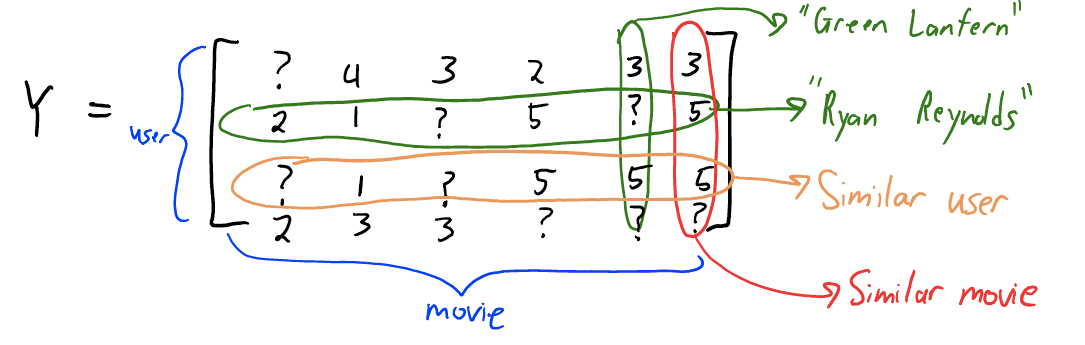
\includegraphics[scale=0.1]{user-item_matrix}
\begin{itemize}
    \item unsupervised learning --- only use labels
    \item latent-factor model: \(y_{ij} \approx w_j^\intercal z_i\)
    \begin{itemize}
        \item \(z_{ic}\) =  ``likes romantic comedies''
        \item \(w_{ic}\) =  ``has Nicholas Cage''
    \end{itemize}
    \item loss function: \(f(Z,W) = \sum\limits_{(i,j) \in R} (w_j^\intercal - y_{ij})^2 + \frac{\lambda_1}{2} ||Z||_F^2 + \frac{\lambda_2}{2} ||W||_F^2\)
    \item add biases: \(y_{ij} \approx \beta + \beta_i + \beta_j + w_j^\intercal z_i\)
    \begin{itemize}
        \item \(\beta \) = global bias
        \item \(\beta_i \) = user-specific bias
        \item \(\beta_j \) = user-specific bias
    \end{itemize}
    \item \(Y_{n \times d} \approx Z_{n \times k} W_{k \times d}\)
\end{itemize}

\subsection{Note}
Problems:
\begin{itemize}
    \item diversity --- how different are the recommendations?
    \item persistence --- how long should recommendations last?
    \item trust --- tell user why you made a recommendation
    \item social recommendation --- what did your friends watch?
    \item freshness --- new and surprising things
\end{itemize}
Content-Based vs. Collaborative
\begin{itemize}
    \item content-based is a linear model and collaborative is a latent-factor model
    \item content-based can predict  on new users/movies, but can't learn about each user/movie
    \item collaborative can learn about each user/movie, but can't predict on new users/movies
\end{itemize}

\section{Multi-Dimensional Scaling (MDS)}
Default Objective
\begin{dmath*}
   f(Z) = \sum_{i=1}^{n} \sum_{j=i+1}^{n} (||z_i - z_j|| - ||x_i - x_j||)^2
\end{dmath*}
Better Objective
\begin{dmath*}
    f(Z) = \sum\limits_{i=1}^{n}\sum\limits_{j=i+1}^{n} d_3(d_2(z_i, z_j) - d_1(x_i, x_j))
\end{dmath*}
\begin{itemize}
    \item \(d_1\) = high-dimensional distance to match
    \item \(d_2\) = low-dimensional distance to control
    \item \(d_3\) = controls how we compare high/low-dimensional distances
\end{itemize}
Choosing \(d_1\), \(d_2\), and \(d_3\)
\begin{itemize}
    \item classic MDS: \(d_1(x_i, x_j) = x_i^\intercal x_j\) and \(d_2(z_i, z_j) = z_i^\intercal z_j\)
    \begin{itemize}
        \item obtains PCA for centered \(x_i\)
        \item not good because it's a linear model
    \end{itemize}
    \item alternative: \(d_1(x_i, x_j) = ||x_i - x_j||_1\) and \(d_2(z_i, z_j) = ||z_i - z_j||\)
    \begin{itemize}
        \item \(z_i\) approximates high-dimensional L1-norm distances
    \end{itemize}
    \item Sammon's mapping to make MDS less crowded by using \emph{weighted} MDS
    \begin{itemize}
        \item \(f(Z) = \sum_{i=1}^{n} \sum_{j=i+1}^{n} (\frac{d_2(z_i,z_j) - d_1(x_i,x_j)}{d_1(x_i,x_j)})^2\)
        \item denominator reduces focus on large distances
    \end{itemize}
\end{itemize}

\subsection{Note}
Main Challenge: crowding effect since it focuses on large distances and loses local structure

\section{ISOMAP}
\begin{center}
    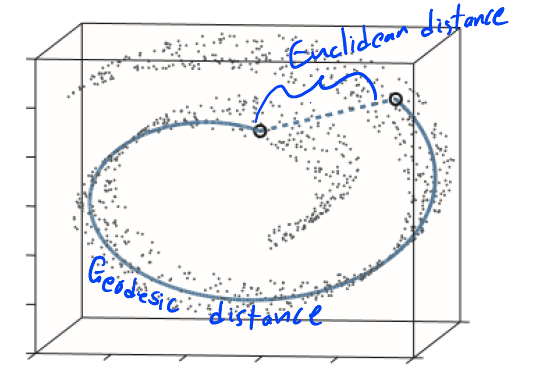
\includegraphics[scale=0.2]{manifold}
\end{center}
\begin{itemize}
    \item PCA/MDS can't discover non-linear manifolds
    \item Geodesic distance (distance through the manifold), is used for low-dimensional manifold
    \item ISOMAP is a latent-factor model for visualizing data on manifolds
\end{itemize}
ISOMAP Procedure \\
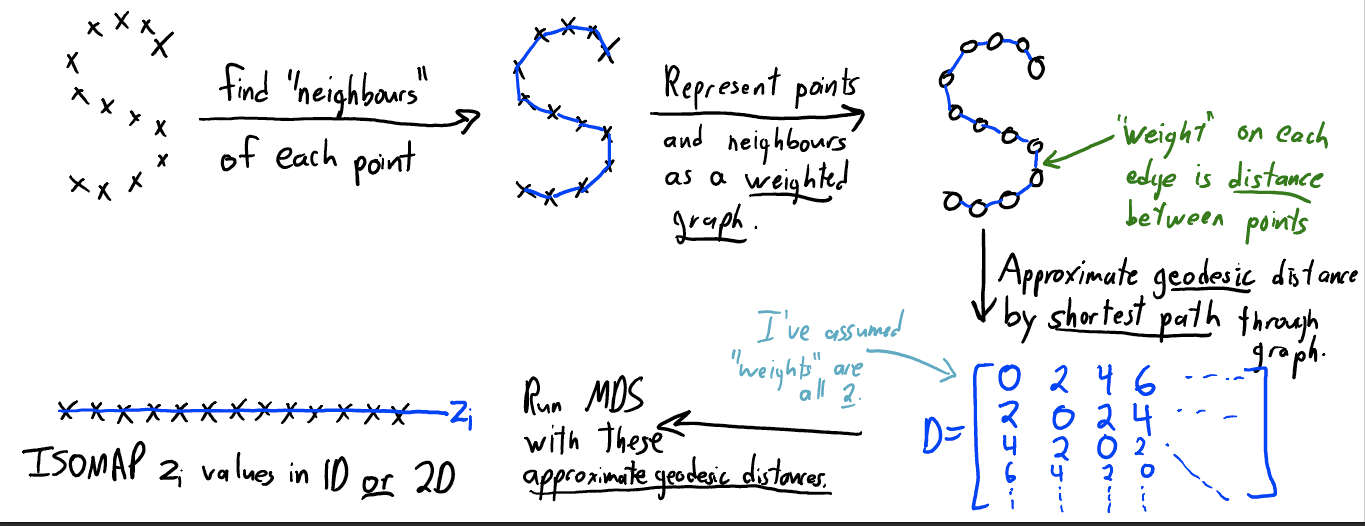
\includegraphics[scale=0.12]{isomap_procedure}

\subsection{Note}
Constructing Neighbour Graph
\begin{itemize}
    \item epsilon graph: convert \(x_i\) to all \(x_j\) within some threshold \(\epsilon \)
    \item KNN graph: connect \(x_i\) to \(x_j\) if \(x_j\) = KNN of \(x_i\) OR \(x_i\) = KNN of \(x_j\)
    \item mutual KNN graph: connect \(x_i\) to \(x_j\) if \(x_j\) = KNN of \(x_i\) AND \(x_i\) = KNN of \(x_j\)
\end{itemize}
ISOMAP vs. t-SNE \\
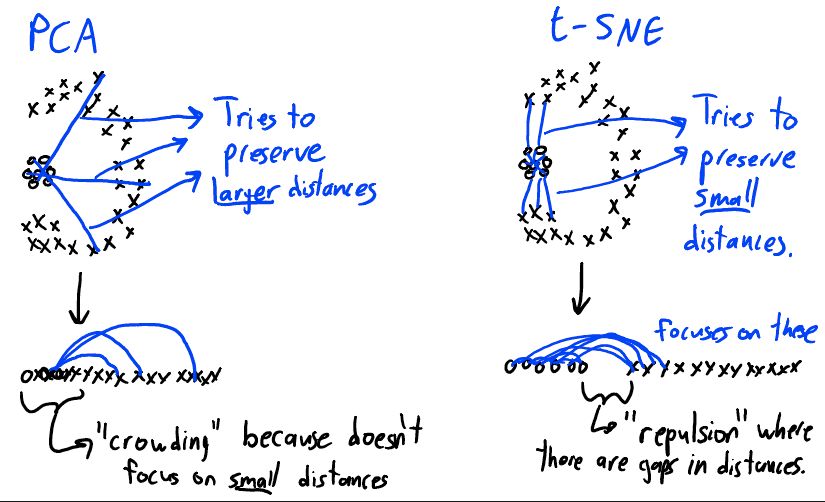
\includegraphics[scale=0.15]{isomap_vs_t-sne}

\section{Neural Networks}

\subsection{Deep Learning}
\begin{center}
    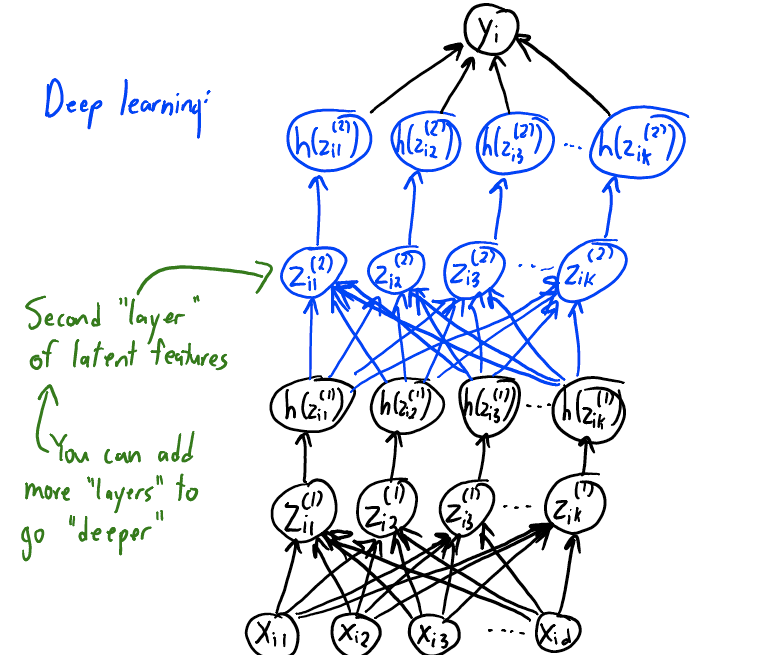
\includegraphics[scale=0.15]{2_hidden_layer_deep_learning}
\end{center}
\begin{dmath*}
    f(W^{(1)},W^{(2)}) = \frac{1}{2} \sum_{i=i}^{n} (w^\intercal h (\underbrace{W^{(2)}h(\underbrace{W^{(1)}x_i}_{z_i^{(1)}}}_{z_i^{(2)}}))-y_i)^2 + \frac{\lambda}{2}||w||^2 + \frac{\lambda_1}{2} ||W^{(1)}||_F^2 + \frac{\lambda_2}{2} ||W^{(2)}||_F^2
\end{dmath*}
\begin{itemize}
    \item \(W^1\) is \(k_1 \times d\), \(W^2\) is \(k_2 \times k_1\), and \(w\) is \(k_2 \times 1\)
    \item \(k \uparrow \) \(\rightarrow \) \(E_{train} \downarrow \text{ but } E_{approx} \uparrow \)
    \item \(\lambda \uparrow \) \(\rightarrow \) \(E_{train} \uparrow \text{ but } E_{approx} \downarrow \)
    \item depth \(\uparrow \) \(\rightarrow \) \(E_{train} \uparrow \text{ but } E_{approx} \downarrow \)
\end{itemize}
Adding Bias Variables
\begin{itemize}
    \item \(y_i = \sum\limits_{c=1}^{k} w_c h(W_c x_i + \beta_c) + \beta\)
    \item bias toward \(h(z_{ic})\) is either 0 or 1
\end{itemize}
Backpropagation
\begin{itemize}
    \item objective function: \(f(w,W) = \frac{1}{2} \sum\limits_{i=1}^{n} (w^\intercal h(W x_i) - y_i)^2\)
    \item compute gradient of random example \(i\), update both \(w\) and \(W\)
    \item highly non-convex and difficult to tune
    \item cost of backpropagation:
    \begin{itemize}
        \item forward pass (\(m\) layers, all \(z_i\) have \(k\) elements): \(O(dk + mk^2)\)
        \item backward pass: same as forward pass
    \end{itemize}
    \item insights
    \begin{itemize}
        \item local minima are \emph{not} a problem
        \item if deep and wide enough, all local minima are good
        \item hard to get SG to find a local minimum
    \end{itemize}
\end{itemize}
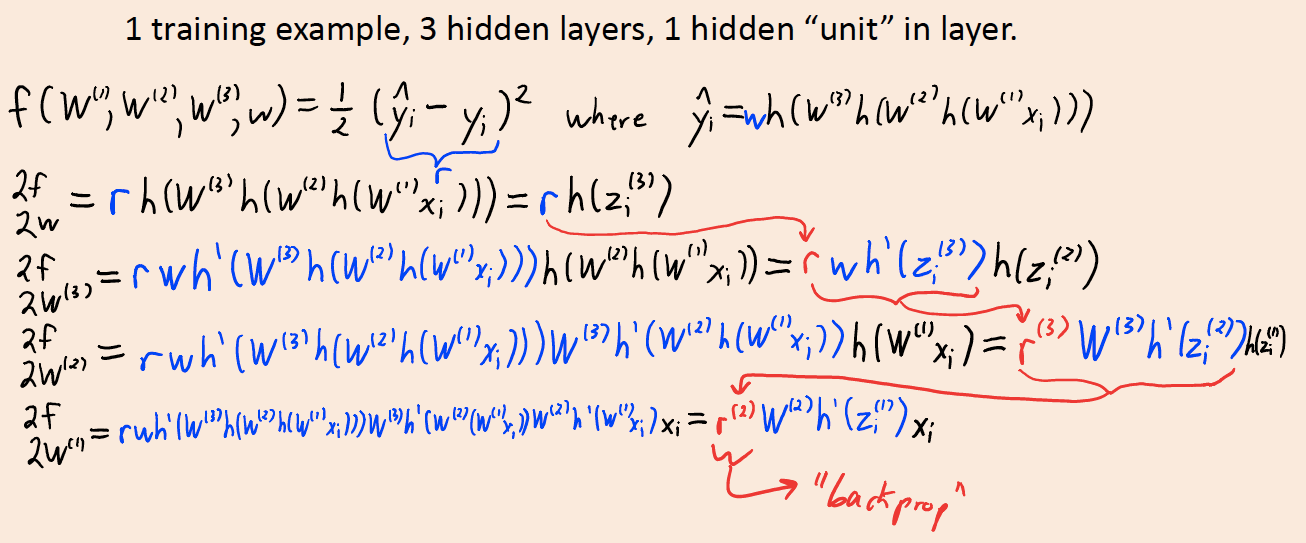
\includegraphics[scale=0.12]{backpropagation} \\
Parameter Initialization
\begin{itemize}
    \item cautions:
    \begin{itemize}
        \item can't initialize weights in same layer to same value, or they will stay the same
        \item can't initialize weights too large, it will take too long to learn
    \end{itemize}
    \item traditional random initialization:
    \begin{itemize}
        \item initialize bias variables to 0
        \item sample from standard normal divided by \(10^5\)
        \begin{itemize}
            \item \(w = 0.0001 \times randon(k, 1)\)
        \end{itemize}
        \item performing multiple initializations are \emph{not} important
    \end{itemize}
    \item recent initializations:
    \begin{itemize}
        \item standardize initial \(z_i\)
        \item different initialization in each layer
        \item make variance of \(z_i\) the same across layers
    \end{itemize}
\end{itemize}
Setting Step-Size
\begin{itemize}
    \item manual babysitting
    \begin{enumerate}
        \item run SG with a fixed step-size
        \item occasionally measure error
        \item if error not deceasing, decrease step-size
    \end{enumerate}
    \item bias step-size multiplier: use bigger step-size for bias variables
    \item momentum (usually \(\beta^t = 0.9\))
    \begin{dmath*}
        w^{t+1} = w^t - \alpha^t \nabla f_i(w^t) + \underbrace{\beta^t (w^t - w^{t-1})}_{\text{adds previous direction}}
    \end{dmath*}
\end{itemize}
Vanishing Gradient Problem
\begin{itemize}
    \item in sigmoid, away from the origin, the gradient is nearly zero
    \item gradients nearly zero everywhere in deep networks
    \item solution: hinge-like loss (ReLU)
\end{itemize}
Trade-off
\begin{itemize}
    \item depth \(\uparrow \rightarrow \) \(E_{train} \downarrow \text{ but } E_{approx} \uparrow\)
\end{itemize}
Regularization
\begin{itemize}
    \item L2 regularization: \(f(w, W^{(3)}, W^{(2)}, W^{(1)}) = \frac{1}{2} \sum\limits_{i=1}^{n} (w^\intercal h(W^{(3)} h(W^{(2)} h(W^{(1)} x_i))) - y_i)^2\)
    \item hyper-parameter optimization: optimize \(E_{validation}\) in terms of \(\lambda_1, \lambda_2, \lambda_3, \lambda_4\)
    \item early stopping
    \begin{enumerate}
        \item monitor \(E_{valid}\) while running SG
        \item stop if \(E_{valid}\) starts increasing
    \end{enumerate}
\end{itemize}

\subsection{Convolutional Neural Networks}
Motivation:
\begin{itemize}
    \item reduce \# parameters
    \item exploit structure in data
    \item reduce overfitting
\end{itemize}
1D Convolution
\begin{itemize}
    \item input: \(x\) vector of length \(n\)
    \item filter: \(w\) vector of length \(2m+1\)
    \item output: \(z\) vector of length \(n\)
    \begin{itemize}
        \item \(z_i = \sum\limits_{j=-m}^{m} w_j x_{i+j}\)
    \end{itemize}
\end{itemize}
1D Convolution Example \\
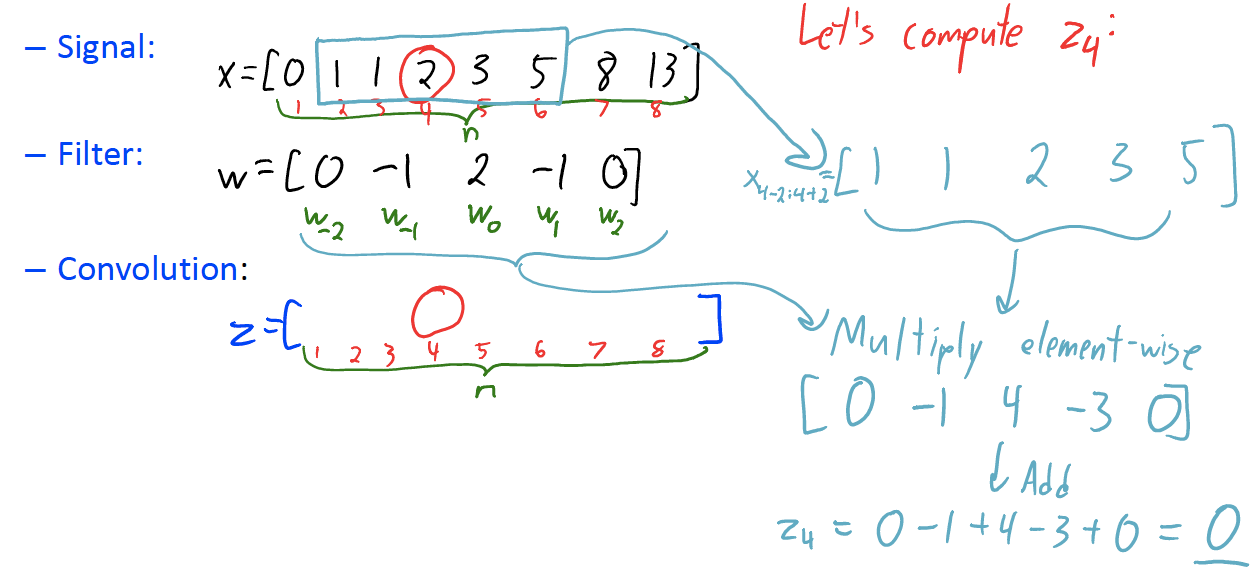
\includegraphics[scale=0.12]{1d_convolution_example}
Boundary Issue Solution
\begin{itemize}
    \item just ignore and return a shorter vector
    \item assign values past boundaries \\
    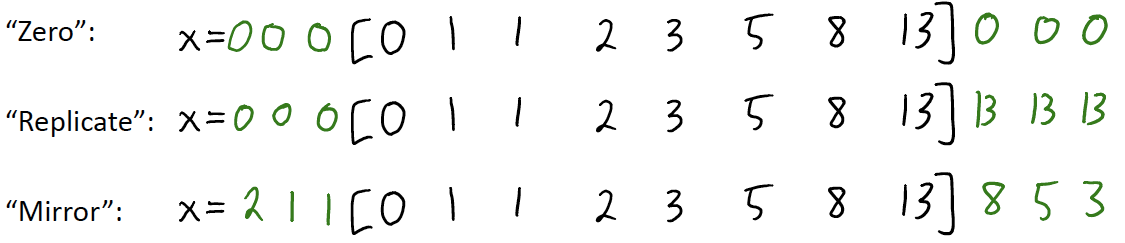
\includegraphics[scale=0.12]{past_boundaries}
\end{itemize}
Convolution as Matrix Multiplication \\
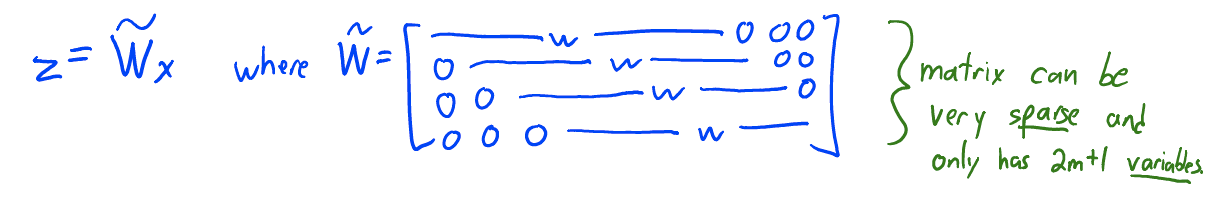
\includegraphics[scale=0.12]{convolution_as_matrix_multiplication}
\begin{itemize}
    \item the shorter \(w\), the more sparse the matrix
\end{itemize}
Three Types of Layers
\begin{itemize}
    \item fully connected: usual neural network layer with unrestricted \(W\) \\
    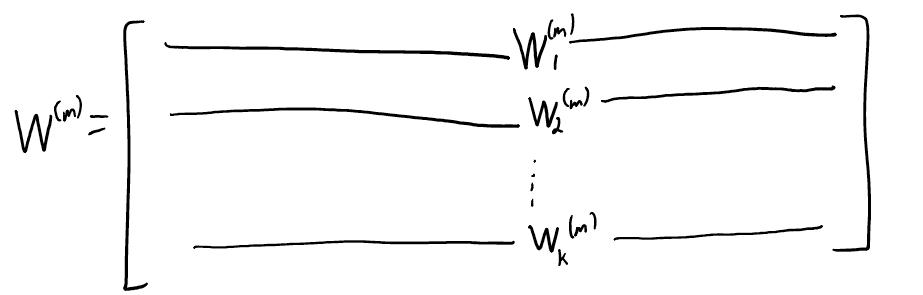
\includegraphics[scale=0.1]{fully_connected}
    \item convolutional: restrict \(W\) to results of several convolutions \\
    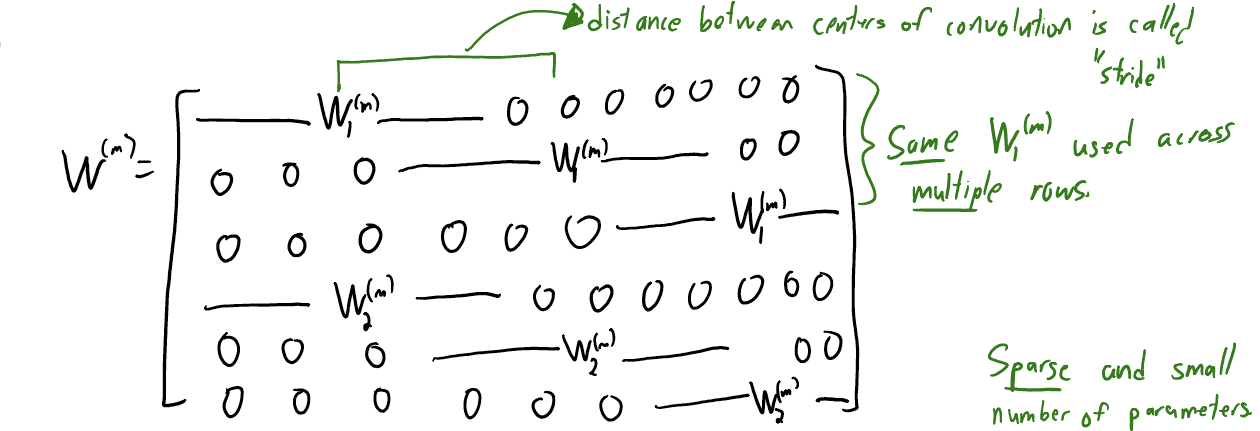
\includegraphics[scale=0.1]{convolutional}
    \item pooling: combine results of convolutions (e.g. max pooling) \\
    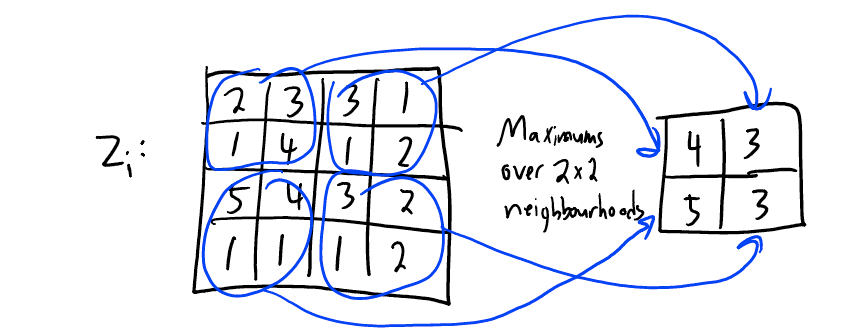
\includegraphics[scale=0.1]{max_pooling}
\end{itemize}

\subsection{\emph{Note}}
Why Sigmoid for \(h(z_i)\)
\begin{itemize}
    \item each \(h(z_i\) can be viewed as a binary feature
    \item sigmoid is a smooth approximation to binary features
\end{itemize}
Deep learning is sensitive to initialization \(\because\) it's non-convex

\section{Math}
Norms:
\begin{itemize}
    \item \(L_2\) or ``Euclidean'' norm
    \begin{equation*}
         ||r||_2 = \sqrt{\sum_{j=1}^{d} r_j^2}
    \end{equation*}
    \item \(L_1\) or ``Manhattan'' norm
    \begin{equation*}
        ||r||_1 = \sum_{j=1}^{d} |r_j|
    \end{equation*}
    \item \(L_{\infty}\) or ``max'' norm
    \begin{equation*}
        ||r||_{\infty} = \max_j{\{|r_j|}\}
    \end{equation*}
    \item ``Frobenius'' norm
    \begin{equation*}
        ||W||_F = \sqrt{\sum_{j=1}^{d} \sum_{c=1}^{k} W_{jc}^2}
    \end{equation*}
\end{itemize}
Objective functions and derivatives:
\begin{align*}
   f(x) &= \frac{1}{2}\sum\limits_{i=1}^{n} (w^\intercal x_i - y_i)^2 + \frac{\lambda}{2} \sum\limits_{j=1}^{d} w_j^2 \\
   &= \frac{1}{2} ||Xw-y||^2 + \frac{\lambda}{2} ||w||^2
\end{align*}
\begin{itemize}
    \item \(\sum\limits_{i=1}^{n} (w^\intercal x_i - y_i)^2 = \sum\limits_{i=1}^{n} r_i^2 = r^\intercal r = ||r||^2\)
    \item \(||v|| = \sqrt{\sum\limits_{j=1}^{d} v_j^2}\), \(u^\intercal v = \sum\limits_{j=1}^{d} u_j v_j\)
    \item \(||w||^2 = \sum\limits_{j=1}^{d} w_j^2 = \sum\limits_{j=1}^{d} w_j w_j = w^\intercal w \)
\end{itemize}
\begin{align*}
    f(w) &= \frac{1}{2} (Xw-y)^\intercal (Xw-y) + \frac{\lambda}{2} w^\intercal w \\
    &= \frac{1}{2} w^\intercal X^\intercal Xw - w^\intercal X^\intercal y - \frac{1}{2} y^\intercal y + \frac{\lambda}{2} w^\intercal w \\
    \nabla f(x) &= X^\intercal Xw - X^\intercal y + \lambda w = 0 \\
    & \rightarrow (X^\intercal X + \lambda I) w = X^\intercal y
\end{align*}
\begin{itemize}
    \item \(\nabla_w (c) = 0\), \(\nabla_w (w^\intercal b) = b\), \(\nabla_w (\frac{1}{2} w^\intercal A w = Aw\)
\end{itemize}
\begin{itemize}
    \item if \(f(x) = \cdots \frac{\lambda}{2} \sum\limits_{j=1}^{d} w_j v_j\), then \(f(x) = \cdots \lambda w^\intercal v\) and \(\nabla f(x) = X^\intercal Xw - X^\intercal y + \lambda v = 0\)
\end{itemize}
\begin{align*}
    f(x) &= \sum\limits_{i=1}^{n} z_i |w^\intercal x_i - y_i| + \lambda \max_j |w_j|
\end{align*}
\begin{align*}
    f(w) = ||Z(Xw - y)||_1 + \lambda ||w||_{\infty}
\end{align*}
Convexity:
\begin{itemize}
    \item \(f''(x) \geq 0 \Rightarrow \) convex
    \item a convex function multiplied by a non-negative constant is convex
    \item norms and squared norms are convex
    \item \(\exp()\) is convex
    \item sum of convex functions is convex
    \item max of convex is convex
    \item composition of a convex function and linear function is convex
    \item \emph{BUT} composition of a convex function and another convex function may not be convex
\end{itemize}
Maximum Likelihood Estimation (MLE):
\begin{itemize}
    \item minimizing NLL
    \item \(f(x) = - \sum_{i=1}^{n}\log{(p(y_i|x_i,w))}\)
    \item runtime: \(O(nd)\)
\end{itemize}
\(m\) Layer Deep Learning \\
$y_i = w^\intercal (\composition\limits_{l=1}^{m} h(W^{(l)} x_i))$
Rectified Linear Units (ReLU)
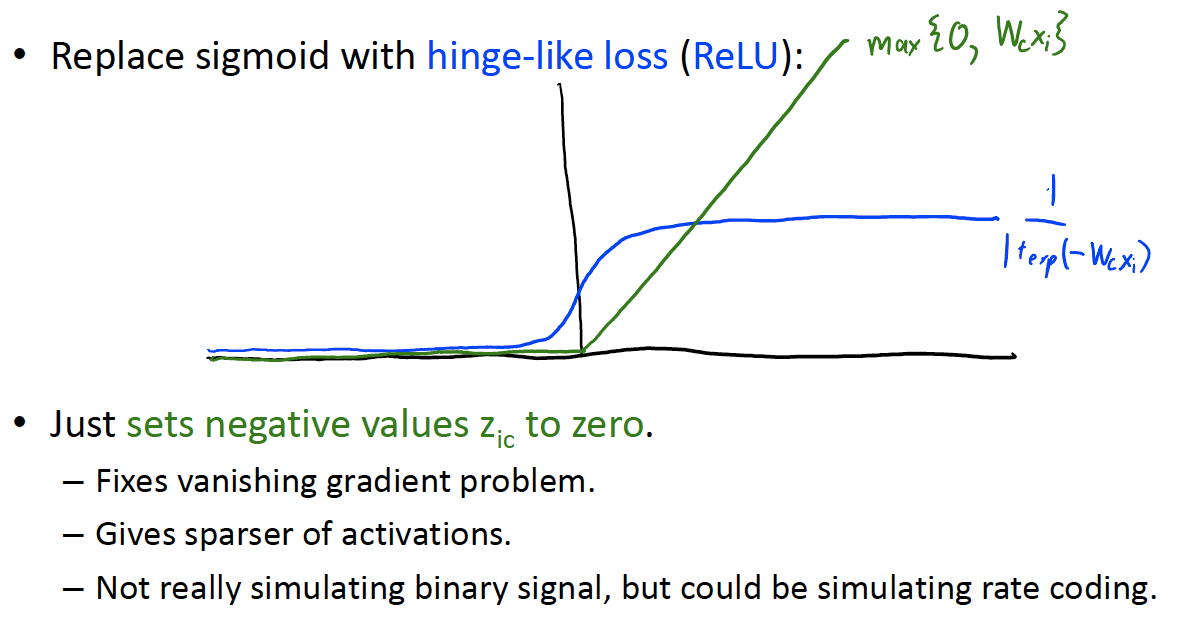
\includegraphics[scale=0.15]{relu}

\section{Plots}
\begin{itemize}
    \item decision tree (1 variable at a time) \\
    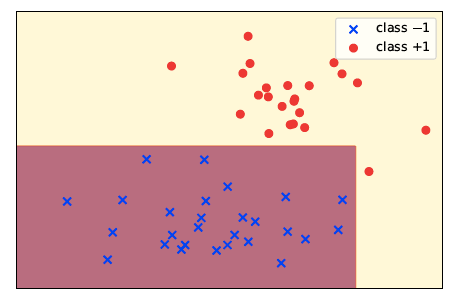
\includegraphics[scale=0.3]{decision_tree_plot}
    \item KNN with \(k=1\) \\
    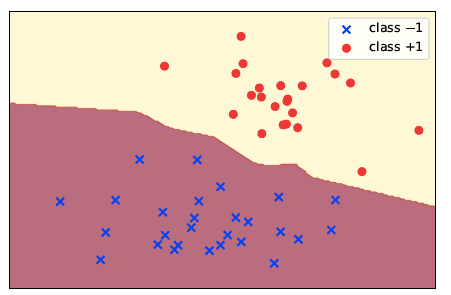
\includegraphics[scale=0.3]{knn_plot}
    \item L2-regularized logistic regression \\
    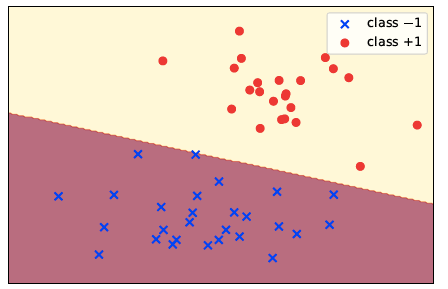
\includegraphics[scale=0.3]{l2_regularized_logistic_regression_plot}
    \item linear SVM (maximizes the margin)\\
    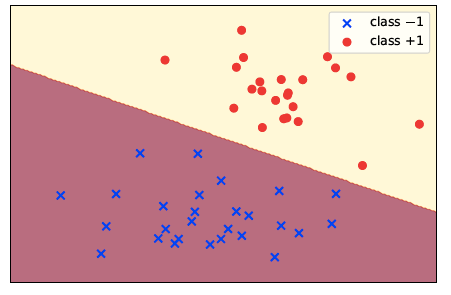
\includegraphics[scale=0.3]{linear_svm_plot}
    \item RBF SVM (blob-like boundaries) \\
    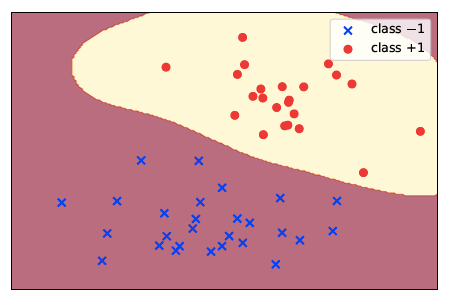
\includegraphics[scale=0.3]{rbf_svm_plot}
    \item neural network using 1 hidden layer and ReLUs \\
    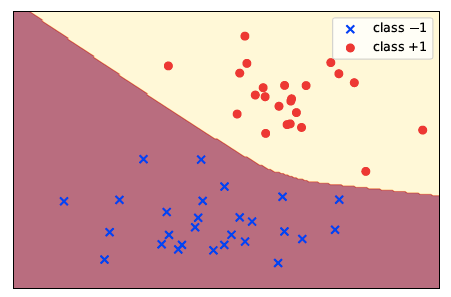
\includegraphics[scale=0.3]{neural_network_plot}
    \item non-regularized L2 norm (not robust) \\
    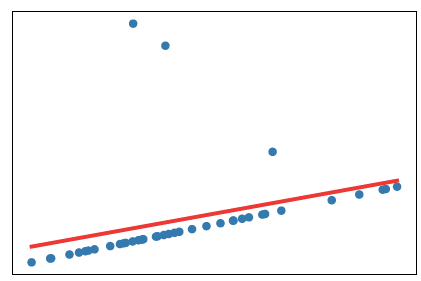
\includegraphics[scale=0.3]{non_regularized_l2_norm}
    \item regularized L2 norm (robust \(\because \) smaller slope) \\
    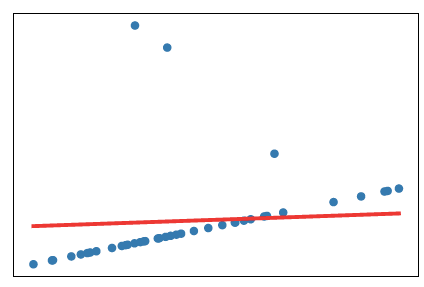
\includegraphics[scale=0.3]{regularized_l2_norm}
    \item L1 norm (robust fit \(\because \) absolute value loss) \\
    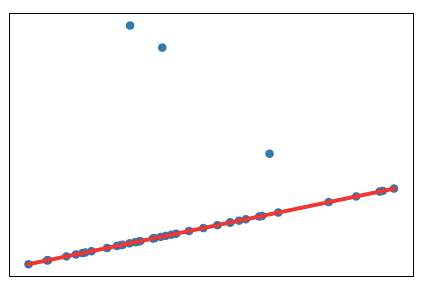
\includegraphics[scale=0.3]{l1_norm}
\end{itemize}

\section{Some Tips}
\begin{itemize}
    \item \textbf{decision stump}: computer error for different stumps then choose the one with the least error
    \item \textbf{randomness of random forest}:
    \begin{itemize}
        \item random subset of data
        \item random subset of features
    \end{itemize}
    \item \textbf{golden rule of ML}: test data should not influence training phase in any way
    \item \textbf{IID assumption}:
    \begin{itemize}
        \item objects from the same distribution
        \item objects sampled independently
    \end{itemize}
    \item \textbf{fundemental trade-off}: \(E_{train} \text{ vs. } E_{approx}\)
    \item \textbf{no free lunch (NFL) theorem}: There is no ``best'' model achieving the best generalization error for every problem.
    \item \textbf{encouraging invariance}: make classifiers invariant to feature transforms by adding transformed data during training
    \item \textbf{removal of outliers}:
    \begin{itemize}
        \item pro: avoid distortion
        \item con: outliers could be real data
    \end{itemize}
    \item \textbf{outlierness ratio}: \(\frac{\text{avg distance of } x_i \text{ to its KNNs}}{\text{avg distane of its neigbours of } x_i \text{ their KNNs}}\)
\end{itemize}

\end{multicols*}
\end{document}
